\documentclass[12pt]{SeminarskiADS}

\begin{document}
\Predmet{Adaptivni diskretni sistemi i neuralne mreže}
\Nastavnik{Prof. dr Miloš Daković}
\Naslov{Naslov seminarskog rada}
\Kandidat{Ime i prezime}
\Indeks{123/2011}
%\Datum{januar 2019.}
\maketitle 

%
% Linija koja počinje znakom % je linija komentara
%

\section{Uvod}

Ovaj dokument je primjer seminarskog rada iz predmeta \emph{Adaptivni diskretni sistemi i neuralne mreže}.

Paragrafe dokumenta odvajamo sa jednim praznim redom. U sekciji \ref{sec:mat} je dat primjer rješavanja kvadratne jednačine.

U Windows okruženju preporučujem korišćenje MiKTeX paketa \cite{Miktex} i editora (okruženja) TeXmaker \cite{TeXmaker} TeXstudio \cite{TexStudio}. Više detalja o samom \LaTeX-u možete naći u \cite{LatexMan,LatexMan2}.



\section{Matematičke formule}
\label{sec:mat}

Ova sekcija sadrži primjer matematičkih formula. Rješavamo kvadratnu jednačinu $x^2-4=0$ po nepoznatoj varijabli $x$.
Jedno rješenje je:
$$ x_1=\sqrt{4}=2 $$ 
a drugo rješenje je:
\begin{equation}
\label{eq:DrugoRj}
x_2=-\sqrt{4}=-2.
\end{equation}
Uočite da je rješenje navedeno u (\ref{eq:DrugoRj}) negativno.

Na sličan način možemo riješiti i jednačinu:
$$ x^2-\frac{4}{9}=0.$$

\subsection{Još formula}
Komplikovane matematičke formule nijesu problem:
$$ A = \left[ \sum\limits_{n=1}^{\infty} 
\frac{n}{1+n^3} \right]^{\frac{1}{p}}$$
\begin{equation}
\label{eq:funkcija}
f(x)=\int_0^x e^{-t^2} dt
\end{equation}

\subsection{Rješavanje linearne jednačine}
Posmatrajmo jednačinu:
$$ 2x-12=0. $$

Pretpostavimo da je $x=4$ rješenje prethodne jednačine.
U tom slučaju je izraz na lijevoj strani jednak $2\cdot 4 -12=-4$ a trebali smo dobiti $0$. To znači da je naša pretpostavka pogrešna i da je treba korigovati. Korekciju dobijamo tako što rezultat $-4$ podijelimo sa koeficijentom uz $x$ u polaznoj jednačini i tu korekciju oduzmemo od našeg pretpostavljenog rješenja, tako da je korigovano rješenje:
$$ x=4-\frac{-4}{2}=6 $$

\section{Grafika}
\label{sec:grafika}

U dokument je često potrebno umetnuti sliku. \LaTeX\ okruženje prepoznaje dva formata slika:
\begin{itemize}
\item EPS format koji se koristi isključivo ako dokument kompajliramo sa latex-om
\item PDF format koji se koristi isključivo ako dokument kompajliramo sa pdflatex-om. U ovom slučaju se pored PDF formata mogu koristiti i slike u formatima JPEG i PNG.
\end{itemize}
Preporučujem da iz Octave ili Matlab okruženja kreirate slike u eps formatu komandom: \verb|print Naziv_slike -depsc|. 
Nakon toga se iz komandnog prozora može izvršiti konverzija slike u PDF format komandom: \verb|epstopdf Naziv_slike.eps|. Ova komanda se može pozvati i direktno iz Matlab-a (sa uzvičnikom ispred).
U komandnom prozoru se može uraditi: \verb|for %1 in (*.eps) do  epstopdf %1|. Ovom komandom će svi EPS fajlovi u tekućem direktorijumu biti konvertovani u PDF format.

Funkcija opisana formulom (\ref{eq:funkcija}) je prikazana na slici \ref{Slika1}.

\begin{figure}[tbp]
\centering
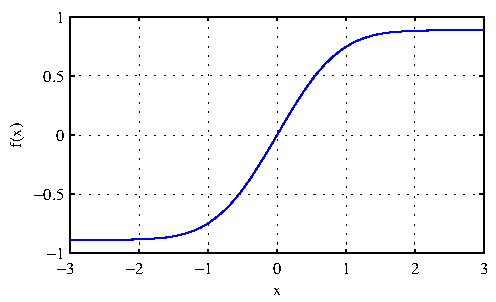
\includegraphics{Slika1}
\caption{Funkcija $f(x)$ definisana jednačinom (\ref{eq:funkcija})}
\label{Slika1}
\end{figure}


\section{Tabele}

Tabele pravimo koristeći okruženja tabular i table.
Primjer ,,floating`` tabele je Tabela \ref{tab:1}.
\begin{table}[tbh]
\caption{Naslov tabele se obično stavlja iznad nje}
\label{tab:1}
\centering
\begin{tabular}{lcl}
\toprule
Funkcija & Formula & Opis \\ 
\midrule 
linearna & $y=ax+b$ & linearna veza $y$ i $x$ \\ 
kvadratna & $y=ax^2+bx+c$ & kvadratna veza $y$ i $x$ \\ 
eksponencijalna & $y=e^{ax}$ & osnova je $e\approx 2,71828183$\\ 
sinusna & $y=A\sin(\omega x+\phi)$ & frekvencija $\omega$ i početna faza $\phi$\\ 
\bottomrule
\end{tabular} 
\end{table}


\section{Programi}

U ovoj sekciji su data dva programa korišćena za dobijanje slike \ref{Slika1}. Programi su rađeni u MATLAB okruženju.

\subsection{Funkcija SetFigureDefaults.m}
Funkcija se koristi za zadavanje preciznih dimenzija slike. Širina i dužina koje se zadaju predstavljaju dimenzije samog grafika (okvira u kojem se crta grafik), tako da će konačne dimenzije slike biti nešto veće, u skladu sa tim kakve smo oznake postavili na osama grafika.
\lstinputlisting{SetFigureDefaults.m}

\subsection{Skript fajl Slika1.m}
Ovaj fajl kreira EPS fajl \texttt{Slika1.eps} koji se u PDF format konvertuje na način opisan u sekciji \ref{sec:grafika}.
\lstinputlisting{Slika1.m}


\section*{Zaključak}
\addcontentsline{toc}{section}{Zaključak}

Korišćenje \LaTeX-a nije komplikovano. Na početku zahtijeva malo više truda, ali se taj trud isplati jer su dokumenti dobijeni na ovaj način izuzetno visokog kvaliteta.

Posebno treba napomenuti da je \LaTeX\ okruženje u potpunosti besplatno, da forsira autora da razmišlja o sadržaju dokumenta a ne o njegovom izgledu i da nudi mogućnosti koje su slabo zastupljene u klasičnim ,,What You See Is What You Get`` okruženjima.

Dokumente koji uključuju reference, sadržaj\dots\ potrebno je kompajlirati više puta.

% Literatura na posebnoj stranici
\clearpage
\begin{thebibliography}{99}
\bibitem{Miktex} MiKTeX projekat,\\
\url{http://miktex.org}

\bibitem{TeXmaker} TeXmaker,\\
\url{http://www.xm1math.net/texmaker}

\bibitem{TexStudio} TeXstudio,\\
\url{http://texstudio.sourceforge.net}

\bibitem{LatexMan} T. Oetiker, ``The Not So Short Introduction to \LaTeX2e'',\\ 
\url{http://tobi.oetiker.ch/lshort/lshort.pdf}

\bibitem{LatexMan2} Š. Ungar, ``Ne baš tako kratak uvod u \TeX\ s naglaskom na \LaTeX2e'', 
Sveučilište J.J. Strossmayera, Osijek, 2002.
\end{thebibliography}

\end{document}
